\documentclass[12pt, a4paper]{article}
\usepackage[utf8]{inputenc}
\usepackage{listings}
\usepackage{courier}
\usepackage{fancyhdr}
\usepackage{color}
\usepackage{xcolor}
\usepackage{caption}
\usepackage{graphicx}
\usepackage{url}
\usepackage[titletoc]{appendix}
\usepackage{textcomp}
\usepackage{pdfpages}
\usepackage[colorlinks]{hyperref}
\hypersetup{urlcolor=blue}


\definecolor{light-gray}{gray}{0.95}

\lstset{
 upquote=true,
 showspaces=false,
 showtabs=false,
 frame=none,
 tabsize=2,
 breaklines=true,
 numbers=none,
 showstringspaces=false,
 breakatwhitespace=true,
 escapeinside={(*@}{@*)},
 keywordstyle=\bfseries,
 basicstyle=\footnotesize\ttfamily,
}

\newcommand{\code}[1]{{\footnotesize\texttt{#1}}}

\setlength\parindent{0pt} % Indentazione paragrafi
\setlength{\parskip}{1ex plus 0.5ex minus 0.2ex} % Spaziatura paragrafi


\title{
  
\includegraphics[width=0.8\textwidth]{img/logo.png}~ \\
  Inter-RAT handover (E-UTRAN to UTRAN) \\ \large Computer Networks module - LTE assignment
}
\author{Michele Zanotti}
\date{Spring term 2018}

\pagestyle{fancy}
\fancyhf{}
\lhead{Computer Networks}
\rhead{LTE assignment}
\rfoot{\thepage}

\begin{document}

\maketitle
\begin{figure}[htb]
	\centering
	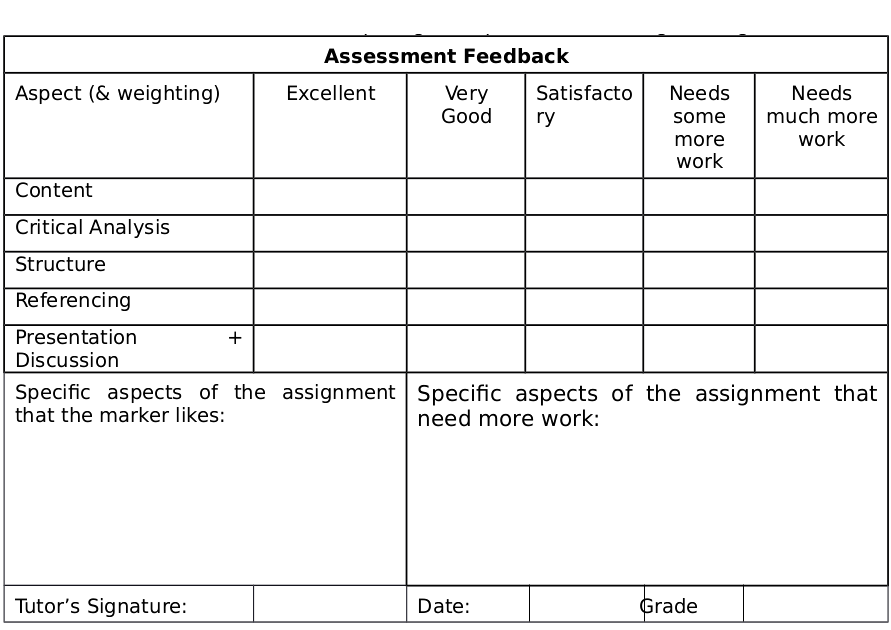
\includegraphics[width=1\linewidth]{img/valuation-table.png}
\end{figure}

\newpage

\section{Introduction}
The intra-RAT handover from E-UTRAN to UTRAN is composed of two phases: the
preparation phase and the execution phase. Both the phases involve either LTE
nodes and UMTS node. In particular, the LTE nodes involved are the eNodeB,
E-UTRAN, and the MME, the S-GW and the P-GW. The first cited node belongs to
the E-UTRAN while the others belong to the core network. The UMTS nodes are instead
the RNC, the SGSN,

\begin{figure}[htb]
	\centering
	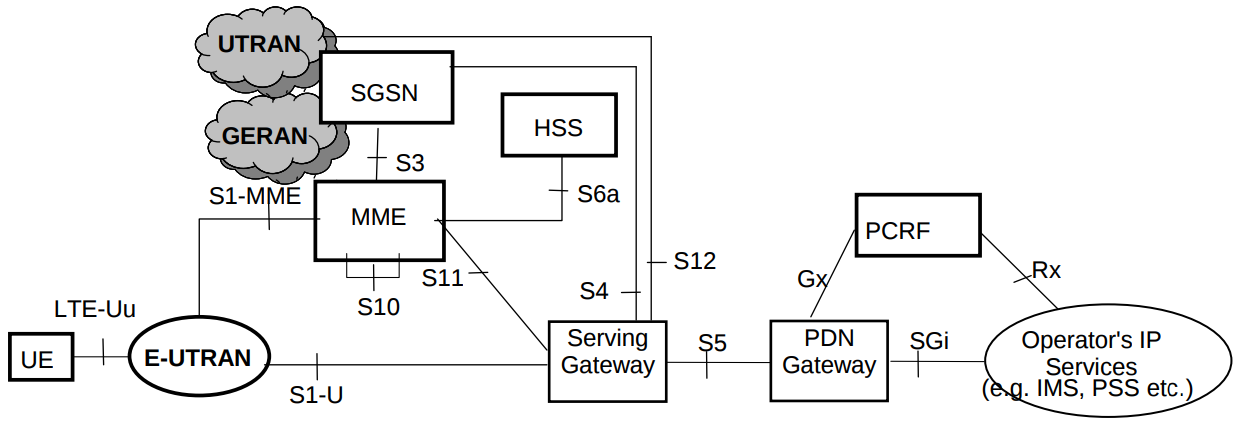
\includegraphics[width=1\linewidth]{img/architecture-reference.png}
	\label{fig:architecture-model}
	\caption{Architecture referece model (non-roaming architecture for 3GPP accesses)}
\end{figure}


\section{Preparation phase}
\begin{figure}[htb]
	\centering
	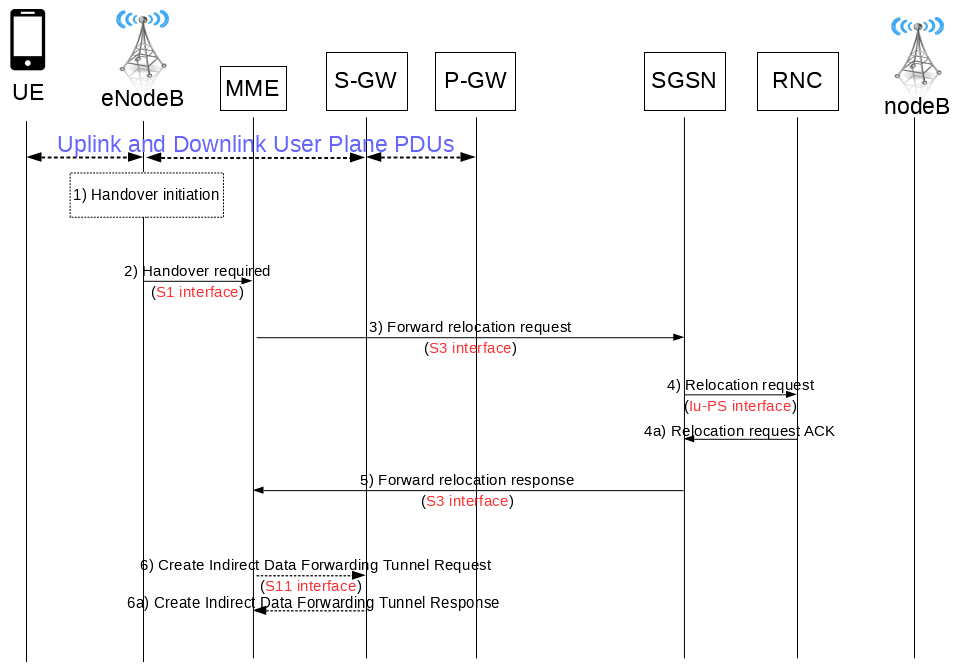
\includegraphics[width=1\linewidth]{img/preparation-phase.png}
	\label{fig:preparation-phase}
	\caption{the flow of the messages and the nodes involved in the
	handover preparation phase}
\end{figure}

\begin{itemize}
	\item [1)] The source eNodeB decides to initiate an Inter-RAT handover to the
	target access network
	\item [2)] The source eNodeB sends a \code{Handover Required} message to the
	source MME, requesting the CN to establish resources in the target RNC,
	target SGSN and the Serving GW. The message is sent through the S1 interface and
	it contains the following parameters:
	\begin{itemize}
		\item S1AP Cause: it specifies the reason of the message
		\item Target RNC Identifier: it identifies the target RNC
		\item CSG access mode: included only if the target cell is a hybrid cell
		\item CSG ID: included only if the target cell is a CSG\footnote{CSG = closed
		subscriber group of a home eNodeB} or hybrid cell, it	identifies the cell
	\end{itemize}
	\item [3)] The source MME determines from the ``Target RNC Identifier'' field that
	the type of handover is intra-RAT Handover to UTRAN Iu mode, then it
	initiates the Handover resource allocation procedure by sending a \code{Forward
	Relocation Request} message to the target SGSN. Some of the parameters included
	in this message are:
	\begin{itemize}
		\item user IMSI
		\item ISR Supported: it indicates if the source MME and the source S-GW are
		able to activate ISR\footnote{ISR = ``idle mode signalling reduction''. When
		this mode is active the network can simultaneously register the UE in a
		routing area that is served by an SGSN and in one or more tracking areas
		that are served by an MME.}
		\item PDN connections: it indicates the active PDN connections
		\item RAN cause: it's the S1AP cause received from the eNodeB
	\end{itemize}


http://www.etsi.org/deliver/etsi_ts/123400_123499/123401/14.07.00_60/ts_123401v140700p.pdf




\begin{thebibliography}{99}
  \footnotesize


\end{thebibliography}

\end{document}
